\chapter{Lý thuyết trò chơi (Game theory)}

Trong chương này, chúng ta sẽ tập trung vào các trò chơi
hai người chơi không chứa các yếu tố ngẫu nhiên.
Mục tiêu của chúng ta là tìm ra một chiến lược mà chúng ta có thể
tuân theo để thắng trò chơi
bất kể đối thủ làm gì,
nếu một chiến lược như vậy tồn tại.

Hóa ra có một chiến lược chung
cho các trò chơi như vậy,
và chúng ta có thể phân tích các trò chơi bằng cách sử dụng \key{lý thuyết Nim (nim theory)}.
Đầu tiên, chúng ta sẽ phân tích các trò chơi đơn giản trong đó
người chơi lấy que khỏi các đống,
và sau đó, chúng ta sẽ tổng quát hóa chiến lược
được sử dụng trong các trò chơi đó cho các trò chơi khác.

\section{Trạng thái trò chơi (Game states)}

Hãy xem xét một trò chơi ban đầu có
một đống gồm $n$ que.
Người chơi $A$ và $B$ di chuyển luân phiên,
và người chơi $A$ bắt đầu.
Trong mỗi lượt đi, người chơi phải lấy
1, 2 hoặc 3 que khỏi đống,
và người chơi lấy que cuối cùng sẽ thắng trò chơi.

Ví dụ, nếu $n=10$, trò chơi có thể diễn ra như sau:
\begin{itemize}[noitemsep]
\item Người chơi $A$ lấy 2 que (còn lại 8 que).
\item Người chơi $B$ lấy 3 que (còn lại 5 que).
\item Người chơi $A$ lấy 1 que (còn lại 4 que).
\item Người chơi $B$ lấy 2 que (còn lại 2 que).
\item Người chơi $A$ lấy 2 que và thắng.
\end{itemize}

Trò chơi này bao gồm các trạng thái $0,1,2,\ldots,n$,
trong đó số của trạng thái tương ứng với
số que còn lại.

\subsubsection{Trạng thái thắng và thua}

\index{winning state}
\index{losing state}

Một \key{trạng thái thắng (winning state)} là một trạng thái mà
người chơi sẽ thắng trò chơi nếu họ
chơi một cách tối ưu,
và một \key{trạng thái thua (losing state)} là một trạng thái
mà người chơi sẽ thua trò chơi nếu
đối thủ chơi một cách tối ưu.
Hóa ra chúng ta có thể phân loại tất cả các trạng thái
của một trò chơi sao cho mỗi trạng thái hoặc là
một trạng thái thắng hoặc là một trạng thái thua.

Trong trò chơi trên, trạng thái 0 rõ ràng là một
trạng thái thua, vì người chơi không thể thực hiện
bất kỳ nước đi nào.
Các trạng thái 1, 2 và 3 là các trạng thái thắng,
bởi vì chúng ta có thể lấy 1, 2 hoặc 3 que
và thắng trò chơi.
Trạng thái 4, ngược lại, là một trạng thái thua,
bởi vì bất kỳ nước đi nào cũng dẫn đến một trạng thái
là trạng thái thắng cho đối thủ.

Tổng quát hơn, nếu có một nước đi dẫn
từ trạng thái hiện tại đến một trạng thái thua,
thì trạng thái hiện tại là một trạng thái thắng,
và ngược lại, trạng thái hiện tại là một trạng thái thua.
Sử dụng quan sát này, chúng ta có thể phân loại tất cả các trạng thái
của một trò chơi bắt đầu từ các trạng thái thua nơi
không có nước đi nào khả dĩ.

Các trạng thái $0 \ldots 15$ của trò chơi trên
có thể được phân loại như sau
($W$ biểu thị một trạng thái thắng và $L$ biểu thị một trạng thái thua):
\begin{center}
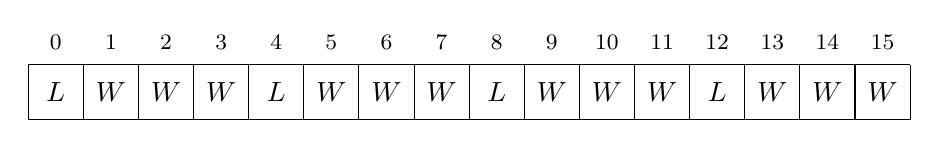
\begin{tikzpicture}[scale=0.7]
\draw (0,0) grid (16,1);

\node at (0.5,0.5) {$L$};
\node at (1.5,0.5) {$W$};
\node at (2.5,0.5) {$W$};
\node at (3.5,0.5) {$W$};
\node at (4.5,0.5) {$L$};
\node at (5.5,0.5) {$W$};
\node at (6.5,0.5) {$W$};
\node at (7.5,0.5) {$W$};
\node at (8.5,0.5) {$L$};
\node at (9.5,0.5) {$W$};
\node at (10.5,0.5) {$W$};
\node at (11.5,0.5) {$W$};
\node at (12.5,0.5) {$L$};
\node at (13.5,0.5) {$W$};
\node at (14.5,0.5) {$W$};
\node at (15.5,0.5) {$W$};

\footnotesize
\node at (0.5,1.4) {$0$};
\node at (1.5,1.4) {$1$};
\node at (2.5,1.4) {$2$};
\node at (3.5,1.4) {$3$};
\node at (4.5,1.4) {$4$};
\node at (5.5,1.4) {$5$};
\node at (6.5,1.4) {$6$};
\node at (7.5,1.4) {$7$};
\node at (8.5,1.4) {$8$};
\node at (9.5,1.4) {$9$};
\node at (10.5,1.4) {$10$};
\node at (11.5,1.4) {$11$};
\node at (12.5,1.4) {$12$};
\node at (13.5,1.4) {$13$};
\node at (14.5,1.4) {$14$};
\node at (15.5,1.4) {$15$};
\end{tikzpicture}
\end{center}

Dễ dàng phân tích trò chơi này:
một trạng thái $k$ là một trạng thái thua nếu $k$
chia hết cho 4, và ngược lại nó
là một trạng thái thắng.
Một cách chơi tối ưu là
luôn chọn một nước đi sao cho sau đó
số que trong đống
chia hết cho 4.
Cuối cùng, sẽ không còn que nào và
đối thủ đã thua.

Tất nhiên, chiến lược này yêu cầu
số que \emph{không} chia hết cho 4
khi đến lượt chúng ta đi.
Nếu nó chia hết, chúng ta không thể làm gì,
và đối thủ sẽ thắng trò chơi nếu
họ chơi một cách tối ưu.

\subsubsection{Đồ thị trạng thái (State graph)}

Bây giờ chúng ta hãy xem xét một trò chơi que khác,
trong đó ở mỗi trạng thái $k$, được phép lấy đi
một số lượng que $x$ bất kỳ sao cho $x$
nhỏ hơn $k$ và là ước của $k$.
Ví dụ, ở trạng thái 8 chúng ta có thể lấy
1, 2 hoặc 4 que, nhưng ở trạng thái 7, nước đi
duy nhất được phép là lấy 1 que.

Hình sau cho thấy các trạng thái
$1 \ldots 9$ của trò chơi dưới dạng một \key{đồ thị trạng thái (state graph)},
có các nút là các trạng thái và các cạnh là các nước đi giữa chúng:

\begin{center}
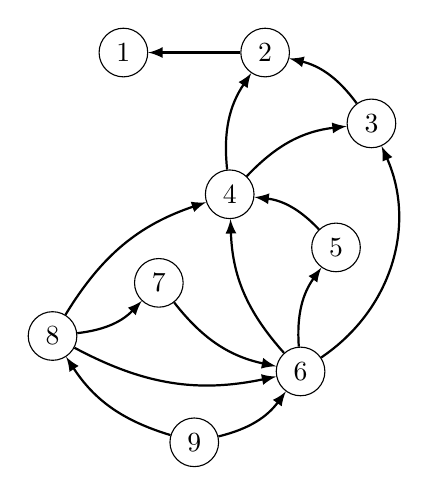
\begin{tikzpicture}[scale=0.9]
\node[draw, circle] (1) at (0,0) {$1$};
\node[draw, circle] (2) at (2,0) {$2$};
\node[draw, circle] (3) at (3.5,-1) {$3$};
\node[draw, circle] (4) at (1.5,-2) {$4$};
\node[draw, circle] (5) at (3,-2.75) {$5$};
\node[draw, circle] (6) at (2.5,-4.5) {$6$};
\node[draw, circle] (7) at (0.5,-3.25) {$7$};
\node[draw, circle] (8) at (-1,-4) {$8$};
\node[draw, circle] (9) at (1,-5.5) {$9$};

\path[draw,thick,->,>=latex] (2) -- (1);
\path[draw,thick,->,>=latex] (3) edge [bend right=20] (2);
\path[draw,thick,->,>=latex] (4) edge [bend left=20] (2);
\path[draw,thick,->,>=latex] (4) edge [bend left=20] (3);
\path[draw,thick,->,>=latex] (5) edge [bend right=20] (4);
\path[draw,thick,->,>=latex] (6) edge [bend left=20] (5);
\path[draw,thick,->,>=latex] (6) edge [bend left=20] (4);
\path[draw,thick,->,>=latex] (6) edge [bend right=40] (3);
\path[draw,thick,->,>=latex] (7) edge [bend right=20] (6);
\path[draw,thick,->,>=latex] (8) edge [bend right=20] (7);
\path[draw,thick,->,>=latex] (8) edge [bend right=20] (6);
\path[draw,thick,->,>=latex] (8) edge [bend left=20] (4);
\path[draw,thick,->,>=latex] (9) edge [bend left=20] (8);
\path[draw,thick,->,>=latex] (9) edge [bend right=20] (6);
\end{tikzpicture}
\end{center}

Trạng thái cuối cùng trong trò chơi này luôn là trạng thái 1,
là một trạng thái thua, vì không có
nước đi hợp lệ nào.
Phân loại các trạng thái $1 \ldots 9$
như sau:

\begin{center}
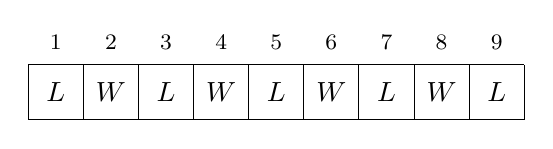
\begin{tikzpicture}[scale=0.7]
\draw (1,0) grid (10,1);

\node at (1.5,0.5) {$L$};
\node at (2.5,0.5) {$W$};
\node at (3.5,0.5) {$L$};
\node at (4.5,0.5) {$W$};
\node at (5.5,0.5) {$L$};
\node at (6.5,0.5) {$W$};
\node at (7.5,0.5) {$L$};
\node at (8.5,0.5) {$W$};
\node at (9.5,0.5) {$L$};

\footnotesize
\node at (1.5,1.4) {$1$};
\node at (2.5,1.4) {$2$};
\node at (3.5,1.4) {$3$};
\node at (4.5,1.4) {$4$};
\node at (5.5,1.4) {$5$};
\node at (6.5,1.4) {$6$};
\node at (7.5,1.4) {$7$};
\node at (8.5,1.4) {$8$};
\node at (9.5,1.4) {$9$};
\end{tikzpicture}
\end{center}

Thật đáng ngạc nhiên, trong trò chơi này,
tất cả các trạng thái có số chẵn đều là trạng thái thắng,
và tất cả các trạng thái có số lẻ đều là trạng thái thua.

\section{Trò chơi Nim (Nim game)}

\index{nim game}

\key{Trò chơi Nim (nim game)} là một trò chơi đơn giản
có vai trò quan trọng trong lý thuyết trò chơi,
bởi vì nhiều trò chơi khác có thể được chơi bằng
cùng một chiến lược.
Đầu tiên, chúng ta tập trung vào nim,
và sau đó chúng ta tổng quát hóa chiến lược
cho các trò chơi khác.

Có $n$ đống trong nim,
và mỗi đống chứa một số lượng que nhất định.
Người chơi đi luân phiên,
và trong mỗi lượt, người chơi chọn
một đống vẫn còn que
và lấy đi một số lượng que bất kỳ từ đó.
Người thắng là người lấy que cuối cùng.

Các trạng thái trong nim có dạng
$[x_1,x_2,\ldots,x_n]$,
trong đó $x_k$ biểu thị số que trong đống $k$.
Ví dụ, $[10,12,5]$ là một trò chơi có
ba đống với 10, 12 và 5 que.
Trạng thái $[0,0,\ldots,0]$ là một trạng thái thua,
bởi vì không thể lấy que nào,
và đây luôn là trạng thái cuối cùng.

\subsubsection{Phân tích}
\index{nim sum}

Hóa ra chúng ta có thể dễ dàng phân loại
bất kỳ trạng thái nim nào bằng cách tính
\key{tổng Nim (nim sum)} $s = x_1 \oplus x_2 \oplus \cdots \oplus x_n$,
trong đó $\oplus$ là phép toán xor\footnote{Chiến lược tối ưu
cho nim được công bố vào năm 1901 bởi C. L. Bouton \cite{bou01}.}.
Các trạng thái có tổng Nim bằng 0 là các trạng thái thua,
và tất cả các trạng thái khác là các trạng thái thắng.
Ví dụ, tổng Nim của
$[10,12,5]$ là $10 \oplus 12 \oplus 5 = 3$,
vì vậy trạng thái này là một trạng thái thắng.

Nhưng tổng Nim liên quan đến trò chơi nim như thế nào?
Chúng ta có thể giải thích điều này bằng cách xem xét cách tổng Nim
thay đổi khi trạng thái nim thay đổi.

\textit{Trạng thái thua:}
Trạng thái cuối cùng $[0,0,\ldots,0]$ là một trạng thái thua,
và tổng Nim của nó là 0, như mong đợi.
Trong các trạng thái thua khác, bất kỳ nước đi nào cũng dẫn đến
một trạng thái thắng, bởi vì khi một giá trị $x_k$ duy nhất thay đổi,
tổng Nim cũng thay đổi, vì vậy tổng Nim
sẽ khác 0 sau nước đi.

\textit{Trạng thái thắng:}
Chúng ta có thể di chuyển đến một trạng thái thua nếu
có bất kỳ đống $k$ nào mà $x_k \oplus s < x_k$.
Trong trường hợp này, chúng ta có thể lấy que khỏi
đống $k$ sao cho nó sẽ chứa $x_k \oplus s$ que,
điều này sẽ dẫn đến một trạng thái thua.
Luôn có một đống như vậy, trong đó $x_k$
có một bit một ở vị trí của bit một
trái nhất của $s$.

Ví dụ, hãy xem xét trạng thái $[10,12,5]$.
Trạng thái này là một trạng thái thắng,
bởi vì tổng Nim của nó là 3.
Do đó, phải có một nước đi dẫn
đến một trạng thái thua.
Tiếp theo chúng ta sẽ tìm ra một nước đi như vậy.

Tổng Nim của trạng thái như sau:

\begin{center}
\begin{tabular}{r|r}
10 & \texttt{1010} \\
12 & \texttt{1100} \\
5 & \texttt{0101} \\
\hline
3 & \texttt{0011} \\
\end{tabular}
\end{center}

Trong trường hợp này, đống có 10 que
là đống duy nhất có một bit một
ở vị trí của bit một
trái nhất của tổng Nim:

\begin{center}
\begin{tabular}{r|r}
10 & \texttt{10\underline{1}0} \\
12 & \texttt{1100} \\
5 & \texttt{0101} \\
\hline
3 & \texttt{00\underline{1}1} \\
\end{tabular}
\end{center}

Kích thước mới của đống phải là
$10 \oplus 3 = 9$,
vì vậy chúng ta sẽ chỉ lấy đi một que.
Sau đó, trạng thái sẽ là $[9,12,5]$,
là một trạng thái thua:

\begin{center}
\begin{tabular}{r|r}
9 & \texttt{1001} \\
12 & \texttt{1100} \\
5 & \texttt{0101} \\
\hline
0 & \texttt{0000} \\
\end{tabular}
\end{center}

\subsubsection{Trò chơi Misère}

\index{misère game}

Trong một \key{trò chơi misère (misère game)}, mục tiêu của trò chơi
là ngược lại,
vì vậy người chơi lấy que cuối cùng
sẽ thua trò chơi.
Hóa ra trò chơi nim misère có thể được
chơi một cách tối ưu gần giống như trò chơi nim tiêu chuẩn.

Ý tưởng là đầu tiên chơi trò chơi misère
giống như trò chơi tiêu chuẩn, nhưng thay đổi chiến lược
vào cuối trò chơi.
Chiến lược mới sẽ được áp dụng trong tình huống
mà mỗi đống sẽ chứa tối đa một que
sau nước đi tiếp theo.

Trong trò chơi tiêu chuẩn, chúng ta nên chọn một nước đi
sau đó có một số chẵn các đống có một que.
Tuy nhiên, trong trò chơi misère, chúng ta chọn một nước đi sao cho
có một số lẻ các đống có một que.

Chiến lược này hoạt động vì một trạng thái mà
chiến lược thay đổi luôn xuất hiện trong trò chơi,
và trạng thái này là một trạng thái thắng, bởi vì
nó chứa chính xác một đống có nhiều hơn một que
nên tổng Nim không phải là 0.

\section{Định lý Sprague–Grundy (Sprague–Grundy theorem)}

\index{Sprague–Grundy theorem}

\key{Định lý Sprague–Grundy (Sprague–Grundy theorem)}\footnote{Định lý được
khám phá độc lập bởi R. Sprague \cite{spr35} và P. M. Grundy \cite{gru39}.} tổng quát hóa
chiến lược được sử dụng trong nim cho tất cả các trò chơi thỏa mãn
các yêu cầu sau:

\begin{itemize}[noitemsep]
\item Có hai người chơi đi luân phiên.
\item Trò chơi bao gồm các trạng thái, và các nước đi có thể
trong một trạng thái không phụ thuộc vào lượt của ai.
\item Trò chơi kết thúc khi một người chơi không thể thực hiện nước đi.
\item Trò chơi chắc chắn sẽ kết thúc sớm hay muộn.
\item Người chơi có thông tin đầy đủ về
các trạng thái và các nước đi được phép, và không có sự ngẫu nhiên trong trò chơi.
\end{itemize}
Ý tưởng là tính cho mỗi trạng thái trò chơi
một số Grundy tương ứng với số que
trong một đống nim.
Khi chúng ta biết các số Grundy của tất cả các trạng thái,
chúng ta có thể chơi trò chơi như trò chơi nim.

\subsubsection{Số Grundy (Grundy numbers)}

\index{Grundy number}
\index{mex function}

\key{Số Grundy (Grundy number)} của một trạng thái trò chơi là
\[\textrm{mex}(\{g_1,g_2,\ldots,g_n\}),\]
trong đó $g_1,g_2,\ldots,g_n$ là các số Grundy của các
trạng thái mà chúng ta có thể di chuyển đến,
và hàm mex cho ra số
không âm nhỏ nhất không có trong tập hợp.
Ví dụ, $\textrm{mex}(\{0,1,3\})=2$.
Nếu không có nước đi nào khả dĩ trong một trạng thái,
số Grundy của nó là 0, vì
$\textrm{mex}(\emptyset)=0$.

Ví dụ, trong đồ thị trạng thái
\begin{center}
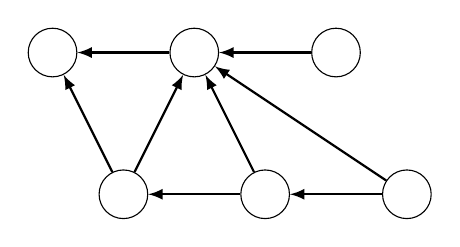
\begin{tikzpicture}[scale=0.9]
\node[draw, circle] (1) at (0,0) {\phantom{0}};
\node[draw, circle] (2) at (2,0) {\phantom{0}};
\node[draw, circle] (3) at (4,0) {\phantom{0}};
\node[draw, circle] (4) at (1,-2) {\phantom{0}};
\node[draw, circle] (5) at (3,-2) {\phantom{0}};
\node[draw, circle] (6) at (5,-2) {\phantom{0}};

\path[draw,thick,->,>=latex] (2) -- (1);
\path[draw,thick,->,>=latex] (3) -- (2);
\path[draw,thick,->,>=latex] (5) -- (4);
\path[draw,thick,->,>=latex] (6) -- (5);
\path[draw,thick,->,>=latex] (4) -- (1);
\path[draw,thick,->,>=latex] (4) -- (2);
\path[draw,thick,->,>=latex] (5) -- (2);
\path[draw,thick,->,>=latex] (6) -- (2);
\end{tikzpicture}
\end{center}
các số Grundy như sau:
\begin{center}
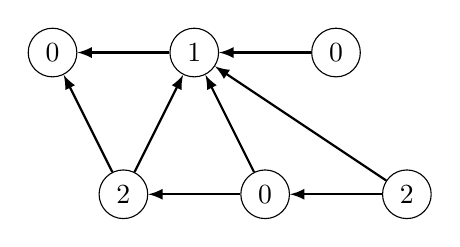
\begin{tikzpicture}[scale=0.9]
\node[draw, circle] (1) at (0,0) {0};
\node[draw, circle] (2) at (2,0) {1};
\node[draw, circle] (3) at (4,0) {0};
\node[draw, circle] (4) at (1,-2) {2};
\node[draw, circle] (5) at (3,-2) {0};
\node[draw, circle] (6) at (5,-2) {2};

\path[draw,thick,->,>=latex] (2) -- (1);
\path[draw,thick,->,>=latex] (3) -- (2);
\path[draw,thick,->,>=latex] (5) -- (4);
\path[draw,thick,->,>=latex] (6) -- (5);
\path[draw,thick,->,>=latex] (4) -- (1);
\path[draw,thick,->,>=latex] (4) -- (2);
\path[draw,thick,->,>=latex] (5) -- (2);
\path[draw,thick,->,>=latex] (6) -- (2);
\end{tikzpicture}
\end{center}
Số Grundy của một trạng thái thua là 0,
và số Grundy của một trạng thái thắng là
một số dương.

Số Grundy của một trạng thái tương ứng với
số que trong một đống nim.
Nếu số Grundy là 0, chúng ta chỉ có thể di chuyển đến
các trạng thái có số Grundy dương,
và nếu số Grundy là $x>0$, chúng ta có thể di chuyển
đến các trạng thái có số Grundy bao gồm tất cả các số
$0,1,\ldots,x-1$.

Ví dụ, hãy xem xét một trò chơi trong đó
người chơi di chuyển một quân cờ trong một mê cung.
Mỗi ô trong mê cung là sàn hoặc tường.
Trong mỗi lượt, người chơi phải di chuyển
quân cờ một số
bước sang trái hoặc lên trên.
Người thắng trò chơi là người
thực hiện nước đi cuối cùng.

Hình sau cho thấy một trạng thái ban đầu có thể có
của trò chơi, trong đó @ biểu thị quân cờ và *
biểu thị một ô mà nó có thể di chuyển đến.

\begin{center}
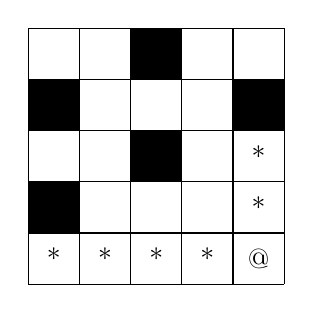
\begin{tikzpicture}[scale=.65]
  \begin{scope}
    \fill [color=black] (0, 1) rectangle (1, 2);
    \fill [color=black] (0, 3) rectangle (1, 4);
    \fill [color=black] (2, 2) rectangle (3, 3);
    \fill [color=black] (2, 4) rectangle (3, 5);
    \fill [color=black] (4, 3) rectangle (5, 4);

    \draw (0, 0) grid (5, 5);
    
    \node at (4.5,0.5) {@};
    \node at (3.5,0.5) {*};
    \node at (2.5,0.5) {*};
    \node at (1.5,0.5) {*};
    \node at (0.5,0.5) {*};
    \node at (4.5,1.5) {*};
    \node at (4.5,2.5) {*};
    
  \end{scope}
\end{tikzpicture}
\end{center}

Các trạng thái của trò chơi là tất cả các ô sàn
của mê cung.
Trong mê cung trên, các số Grundy
như sau:

\begin{center}
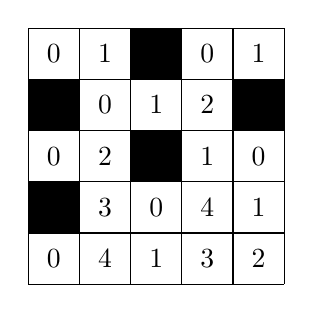
\begin{tikzpicture}[scale=.65]
  \begin{scope}
    \fill [color=black] (0, 1) rectangle (1, 2);
    \fill [color=black] (0, 3) rectangle (1, 4);
    \fill [color=black] (2, 2) rectangle (3, 3);
    \fill [color=black] (2, 4) rectangle (3, 5);
    \fill [color=black] (4, 3) rectangle (5, 4);

    \draw (0, 0) grid (5, 5);
    
    \node at (0.5,4.5) {0};
    \node at (1.5,4.5) {1};
    \node at (2.5,4.5) {};
    \node at (3.5,4.5) {0};
    \node at (4.5,4.5) {1};

    \node at (0.5,3.5) {};
    \node at (1.5,3.5) {0};
    \node at (2.5,3.5) {1};
    \node at (3.5,3.5) {2};
    \node at (4.5,3.5) {};

    \node at (0.5,2.5) {0};
    \node at (1.5,2.5) {2};
    \node at (2.5,2.5) {};
    \node at (3.5,2.5) {1};
    \node at (4.5,2.5) {0};

    \node at (0.5,1.5) {};
    \node at (1.5,1.5) {3};
    \node at (2.5,1.5) {0};
    \node at (3.5,1.5) {4};
    \node at (4.5,1.5) {1};

    \node at (0.5,0.5) {0};
    \node at (1.5,0.5) {4};
    \node at (2.5,0.5) {1};
    \node at (3.5,0.5) {3};
    \node at (4.5,0.5) {2};
  \end{scope}
\end{tikzpicture}
\end{center}

Do đó, mỗi trạng thái của trò chơi mê cung
tương ứng với một đống trong trò chơi nim.
Ví dụ, số Grundy cho
ô dưới cùng bên phải là 2,
vì vậy đó là một trạng thái thắng.
Chúng ta có thể đến một trạng thái thua và
thắng trò chơi bằng cách di chuyển
hoặc bốn bước sang trái hoặc
hai bước lên trên.

Lưu ý rằng không giống như trong trò chơi nim ban đầu,
có thể di chuyển đến một trạng thái có
số Grundy lớn hơn số Grundy
của trạng thái hiện tại.
Tuy nhiên, đối thủ luôn có thể chọn một nước đi
hủy bỏ một nước đi như vậy, vì vậy không thể
thoát khỏi một trạng thái thua.

\subsubsection{Trò chơi con (Subgames)}

Tiếp theo chúng ta sẽ giả sử rằng trò chơi của chúng ta bao gồm
các trò chơi con, và trong mỗi lượt, người chơi
đầu tiên chọn một trò chơi con và sau đó là một nước đi trong trò chơi con đó.
Trò chơi kết thúc khi không thể thực hiện bất kỳ nước đi nào
trong bất kỳ trò chơi con nào.

Trong trường hợp này, số Grundy của một trò chơi
là tổng Nim của các số Grundy của các trò chơi con.
Trò chơi có thể được chơi như một trò chơi nim bằng cách tính
tất cả các số Grundy cho các trò chơi con và sau đó là tổng Nim của chúng.

Ví dụ, hãy xem xét một trò chơi bao gồm
ba mê cung.
Trong trò chơi này, trong mỗi lượt, người chơi chọn một
trong các mê cung và sau đó di chuyển quân cờ trong mê cung đó.
Giả sử trạng thái ban đầu của trò chơi như sau:

\begin{center}
\begin{tabular}{ccc}
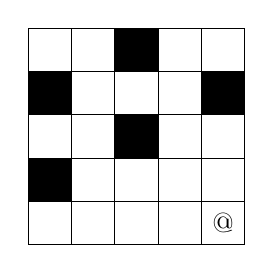
\begin{tikzpicture}[scale=.55]
  \begin{scope}
    \fill [color=black] (0, 1) rectangle (1, 2);
    \fill [color=black] (0, 3) rectangle (1, 4);
    \fill [color=black] (2, 2) rectangle (3, 3);
    \fill [color=black] (2, 4) rectangle (3, 5);
    \fill [color=black] (4, 3) rectangle (5, 4);

    \draw (0, 0) grid (5, 5);

    \node at (4.5,0.5) {@};

    \end{scope}
\end{tikzpicture}
&
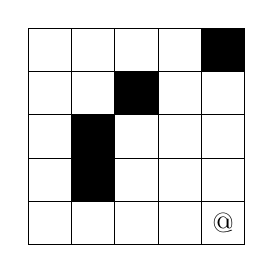
\begin{tikzpicture}[scale=.55]
  \begin{scope}
    \fill [color=black] (1, 1) rectangle (2, 3);
    \fill [color=black] (2, 3) rectangle (3, 4);
    \fill [color=black] (4, 4) rectangle (5, 5);

    \draw (0, 0) grid (5, 5);
    
    \node at (4.5,0.5) {@};

  \end{scope}
\end{tikzpicture}
&
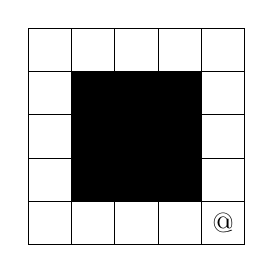
\begin{tikzpicture}[scale=.55]
  \begin{scope}
    \fill [color=black] (1, 1) rectangle (4, 4);

    \draw (0, 0) grid (5, 5);
    
    \node at (4.5,0.5) {@};
  \end{scope}
\end{tikzpicture}
\end{tabular}
\end{center}

Các số Grundy cho các mê cung như sau:

\begin{center}
\begin{tabular}{ccc}
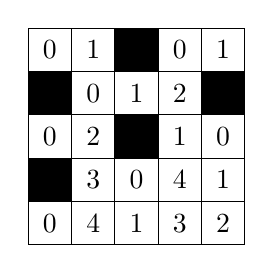
\begin{tikzpicture}[scale=.55]
  \begin{scope}
    \fill [color=black] (0, 1) rectangle (1, 2);
    \fill [color=black] (0, 3) rectangle (1, 4);
    \fill [color=black] (2, 2) rectangle (3, 3);
    \fill [color=black] (2, 4) rectangle (3, 5);
    \fill [color=black] (4, 3) rectangle (5, 4);

    \draw (0, 0) grid (5, 5);

    \node at (0.5,4.5) {0};
    \node at (1.5,4.5) {1};
    \node at (2.5,4.5) {};
    \node at (3.5,4.5) {0};
    \node at (4.5,4.5) {1};

    \node at (0.5,3.5) {};
    \node at (1.5,3.5) {0};
    \node at (2.5,3.5) {1};
    \node at (3.5,3.5) {2};
    \node at (4.5,3.5) {};

    \node at (0.5,2.5) {0};
    \node at (1.5,2.5) {2};
    \node at (2.5,2.5) {};
    \node at (3.5,2.5) {1};
    \node at (4.5,2.5) {0};

    \node at (0.5,1.5) {};
    \node at (1.5,1.5) {3};
    \node at (2.5,1.5) {0};
    \node at (3.5,1.5) {4};
    \node at (4.5,1.5) {1};

    \node at (0.5,0.5) {0};
    \node at (1.5,0.5) {4};
    \node at (2.5,0.5) {1};
    \node at (3.5,0.5) {3};
    \node at (4.5,0.5) {2};
    \end{scope}
\end{tikzpicture}
&
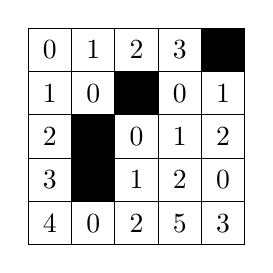
\begin{tikzpicture}[scale=.55]
  \begin{scope}
    \fill [color=black] (1, 1) rectangle (2, 3);
    \fill [color=black] (2, 3) rectangle (3, 4);
    \fill [color=black] (4, 4) rectangle (5, 5);

    \draw (0, 0) grid (5, 5);

    \node at (0.5,4.5) {0};
    \node at (1.5,4.5) {1};
    \node at (2.5,4.5) {2};
    \node at (3.5,4.5) {3};
    \node at (4.5,4.5) {};

    \node at (0.5,3.5) {1};
    \node at (1.5,3.5) {0};
    \node at (2.5,3.5) {};
    \node at (3.5,3.5) {0};
    \node at (4.5,3.5) {1};

    \node at (0.5,2.5) {2};
    \node at (1.5,2.5) {};
    \node at (2.5,2.5) {0};
    \node at (3.5,2.5) {1};
    \node at (4.5,2.5) {2};

    \node at (0.5,1.5) {3};
    \node at (1.5,1.5) {};
    \node at (2.5,1.5) {1};
    \node at (3.5,1.5) {2};
    \node at (4.5,1.5) {0};

    \node at (0.5,0.5) {4};
    \node at (1.5,0.5) {0};
    \node at (2.5,0.5) {2};
    \node at (3.5,0.5) {5};
    \node at (4.5,0.5) {3};
  \end{scope}
\end{tikzpicture}
&
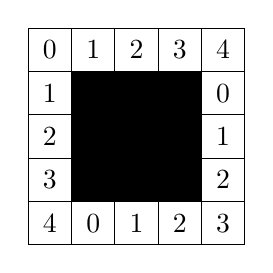
\begin{tikzpicture}[scale=.55]
  \begin{scope}
    \fill [color=black] (1, 1) rectangle (4, 4);

    \draw (0, 0) grid (5, 5);

    \node at (0.5,4.5) {0};
    \node at (1.5,4.5) {1};
    \node at (2.5,4.5) {2};
    \node at (3.5,4.5) {3};
    \node at (4.5,4.5) {4};

    \node at (0.5,3.5) {1};
    \node at (1.5,3.5) {};
    \node at (2.5,3.5) {};
    \node at (3.5,3.5) {};
    \node at (4.5,3.5) {0};

    \node at (0.5,2.5) {2};
    \node at (1.5,2.5) {};
    \node at (2.5,2.5) {};
    \node at (3.5,2.5) {};
    \node at (4.5,2.5) {1};

    \node at (0.5,1.5) {3};
    \node at (1.5,1.5) {};
    \node at (2.5,1.5) {};
    \node at (3.5,1.5) {};
    \node at (4.5,1.5) {2};

    \node at (0.5,0.5) {4};
    \node at (1.5,0.5) {0};
    \node at (2.5,0.5) {1};
    \node at (3.5,0.5) {2};
    \node at (4.5,0.5) {3};
  \end{scope}
\end{tikzpicture}
\end{tabular}
\end{center}

Ở trạng thái ban đầu, tổng Nim của các số Grundy
là $2 \oplus 3 \oplus 3 = 2$, vì vậy
người chơi đầu tiên có thể thắng trò chơi.
Một nước đi tối ưu là di chuyển hai bước lên trên
trong mê cung đầu tiên, tạo ra tổng Nim
$0 \oplus 3 \oplus 3 = 0$.

\subsubsection{Trò chơi của Grundy}

Đôi khi một nước đi trong một trò chơi chia trò chơi
thành các trò chơi con độc lập với nhau.
Trong trường hợp này, số Grundy của trò chơi là

\[\textrm{mex}(\{g_1, g_2, \ldots, g_n \}),\]
trong đó $n$ là số nước đi có thể và
\[g_k = a_{k,1} \oplus a_{k,2} \oplus \ldots \oplus a_{k,m},\]
trong đó nước đi $k$ tạo ra các trò chơi con với
các số Grundy $a_{k,1},a_{k,2},\ldots,a_{k,m}$.

\index{Grundy's game}

Một ví dụ về trò chơi như vậy là \key{trò chơi của Grundy (Grundy's game)}.
Ban đầu, có một đống duy nhất chứa $n$ que.
Trong mỗi lượt, người chơi chọn một đống và chia
nó thành hai đống không rỗng sao cho các đống
có kích thước khác nhau.
Người chơi thực hiện nước đi cuối cùng sẽ thắng trò chơi.

Gọi $f(n)$ là số Grundy của một đống
chứa $n$ que.
Số Grundy có thể được tính bằng cách duyệt
qua tất cả các cách chia đống thành
hai đống.
Ví dụ, khi $n=8$, các khả năng
là $1+7$, $2+6$ và $3+5$, vì vậy
\[f(8)=\textrm{mex}(\{f(1) \oplus f(7), f(2) \oplus f(6), f(3) \oplus f(5)\}).\]

Trong trò chơi này, giá trị của $f(n)$ dựa trên các giá trị
của $f(1),\ldots,f(n-1)$.
Các trường hợp cơ sở là $f(1)=f(2)=0$,
bởi vì không thể chia các đống
có 1 và 2 que.
Các số Grundy đầu tiên là:
\[
\begin{array}{lcl}
f(1) & = & 0 \\
f(2) & = & 0 \\
f(3) & = & 1 \\
f(4) & = & 0 \\
f(5) & = & 2 \\
f(6) & = & 1 \\
f(7) & = & 0 \\
f(8) & = & 2 \\
\end{array}
\]
Số Grundy cho $n=8$ là 2,
vì vậy có thể thắng trò chơi.
Nước đi thắng là tạo ra các đống
$1+7$, vì $f(1) \oplus f(7) = 0$.